\documentclass[xcolor=dvipsnames]{beamer}
\usepackage{fontspec}
\usepackage{graphicx}
\usepackage{xcolor}
\usepackage{tikz}
\setsansfont{Roboto Light}
\graphicspath{{fig/}}

% define color theme
\usecolortheme{dolphin}

% change text to offblack
\definecolor{almostblack}{HTML}{262626}
%\setbeamercolor{normal text}{fg=almostblack}
\setbeamercolor{normal text}{fg=almostblack}

% macros
\newcommand{\trento}{T\raisebox{-0.5ex}{R}ENTo}

\definecolor{theme}{RGB}{90,122,163}
\usecolortheme[named=theme]{structure}

\makeatletter
\setbeamertemplate{frametitle}{
  \ifbeamercolorempty[bg]{frametitle}{}{\nointerlineskip}%
  \@tempdima=\textwidth%
  \advance\@tempdima by\beamer@leftmargin%
  \advance\@tempdima by\beamer@rightmargin%
  \begin{beamercolorbox}[sep=0.3cm,left,wd=\the\@tempdima]{frametitle}
    \vbox{}\vskip-2ex%
    \if@tempswa\else\csname beamer@fteleft\endcsname\fi%
    \strut\insertframetitle\strut\par%
    {%
      \ifx\insertframesubtitle\@empty%
      \else%
      {\usebeamerfont{framesubtitle}\usebeamercolor[fg]{framesubtitle}\insertframesubtitle\strut\par}%
      \fi
    }%
    \vskip.45ex%
    \hrule %height .6pt%
    \vskip-1.45ex%
    \if@tempswa\else\vskip-.3cm\fi%
  \end{beamercolorbox}%
}
\makeatother

% clean up footer
\beamertemplatenavigationsymbolsempty
\setbeamertemplate{footline}[frame number]

%inner theme
\useinnertheme{rectangles}
\setbeamertemplate{itemize item}{\raise.30ex\hbox{\vrule width .80ex height .80ex}}
\setbeamertemplate{itemize subitem}{\raise.35ex\hbox{\vrule width .70ex height .70ex}}

\title{Determining QGP initial conditions and medium properties with Bayesian analysis}
\author{J.S. Moreland, J.E. Bernhard, S.A. Bass}
\date{\today}


\begin{document}

\section{Title}

\usebackgroundtemplate{%
\tikz[overlay,remember picture] \node[opacity=0.4, at=(current page.center)] {
   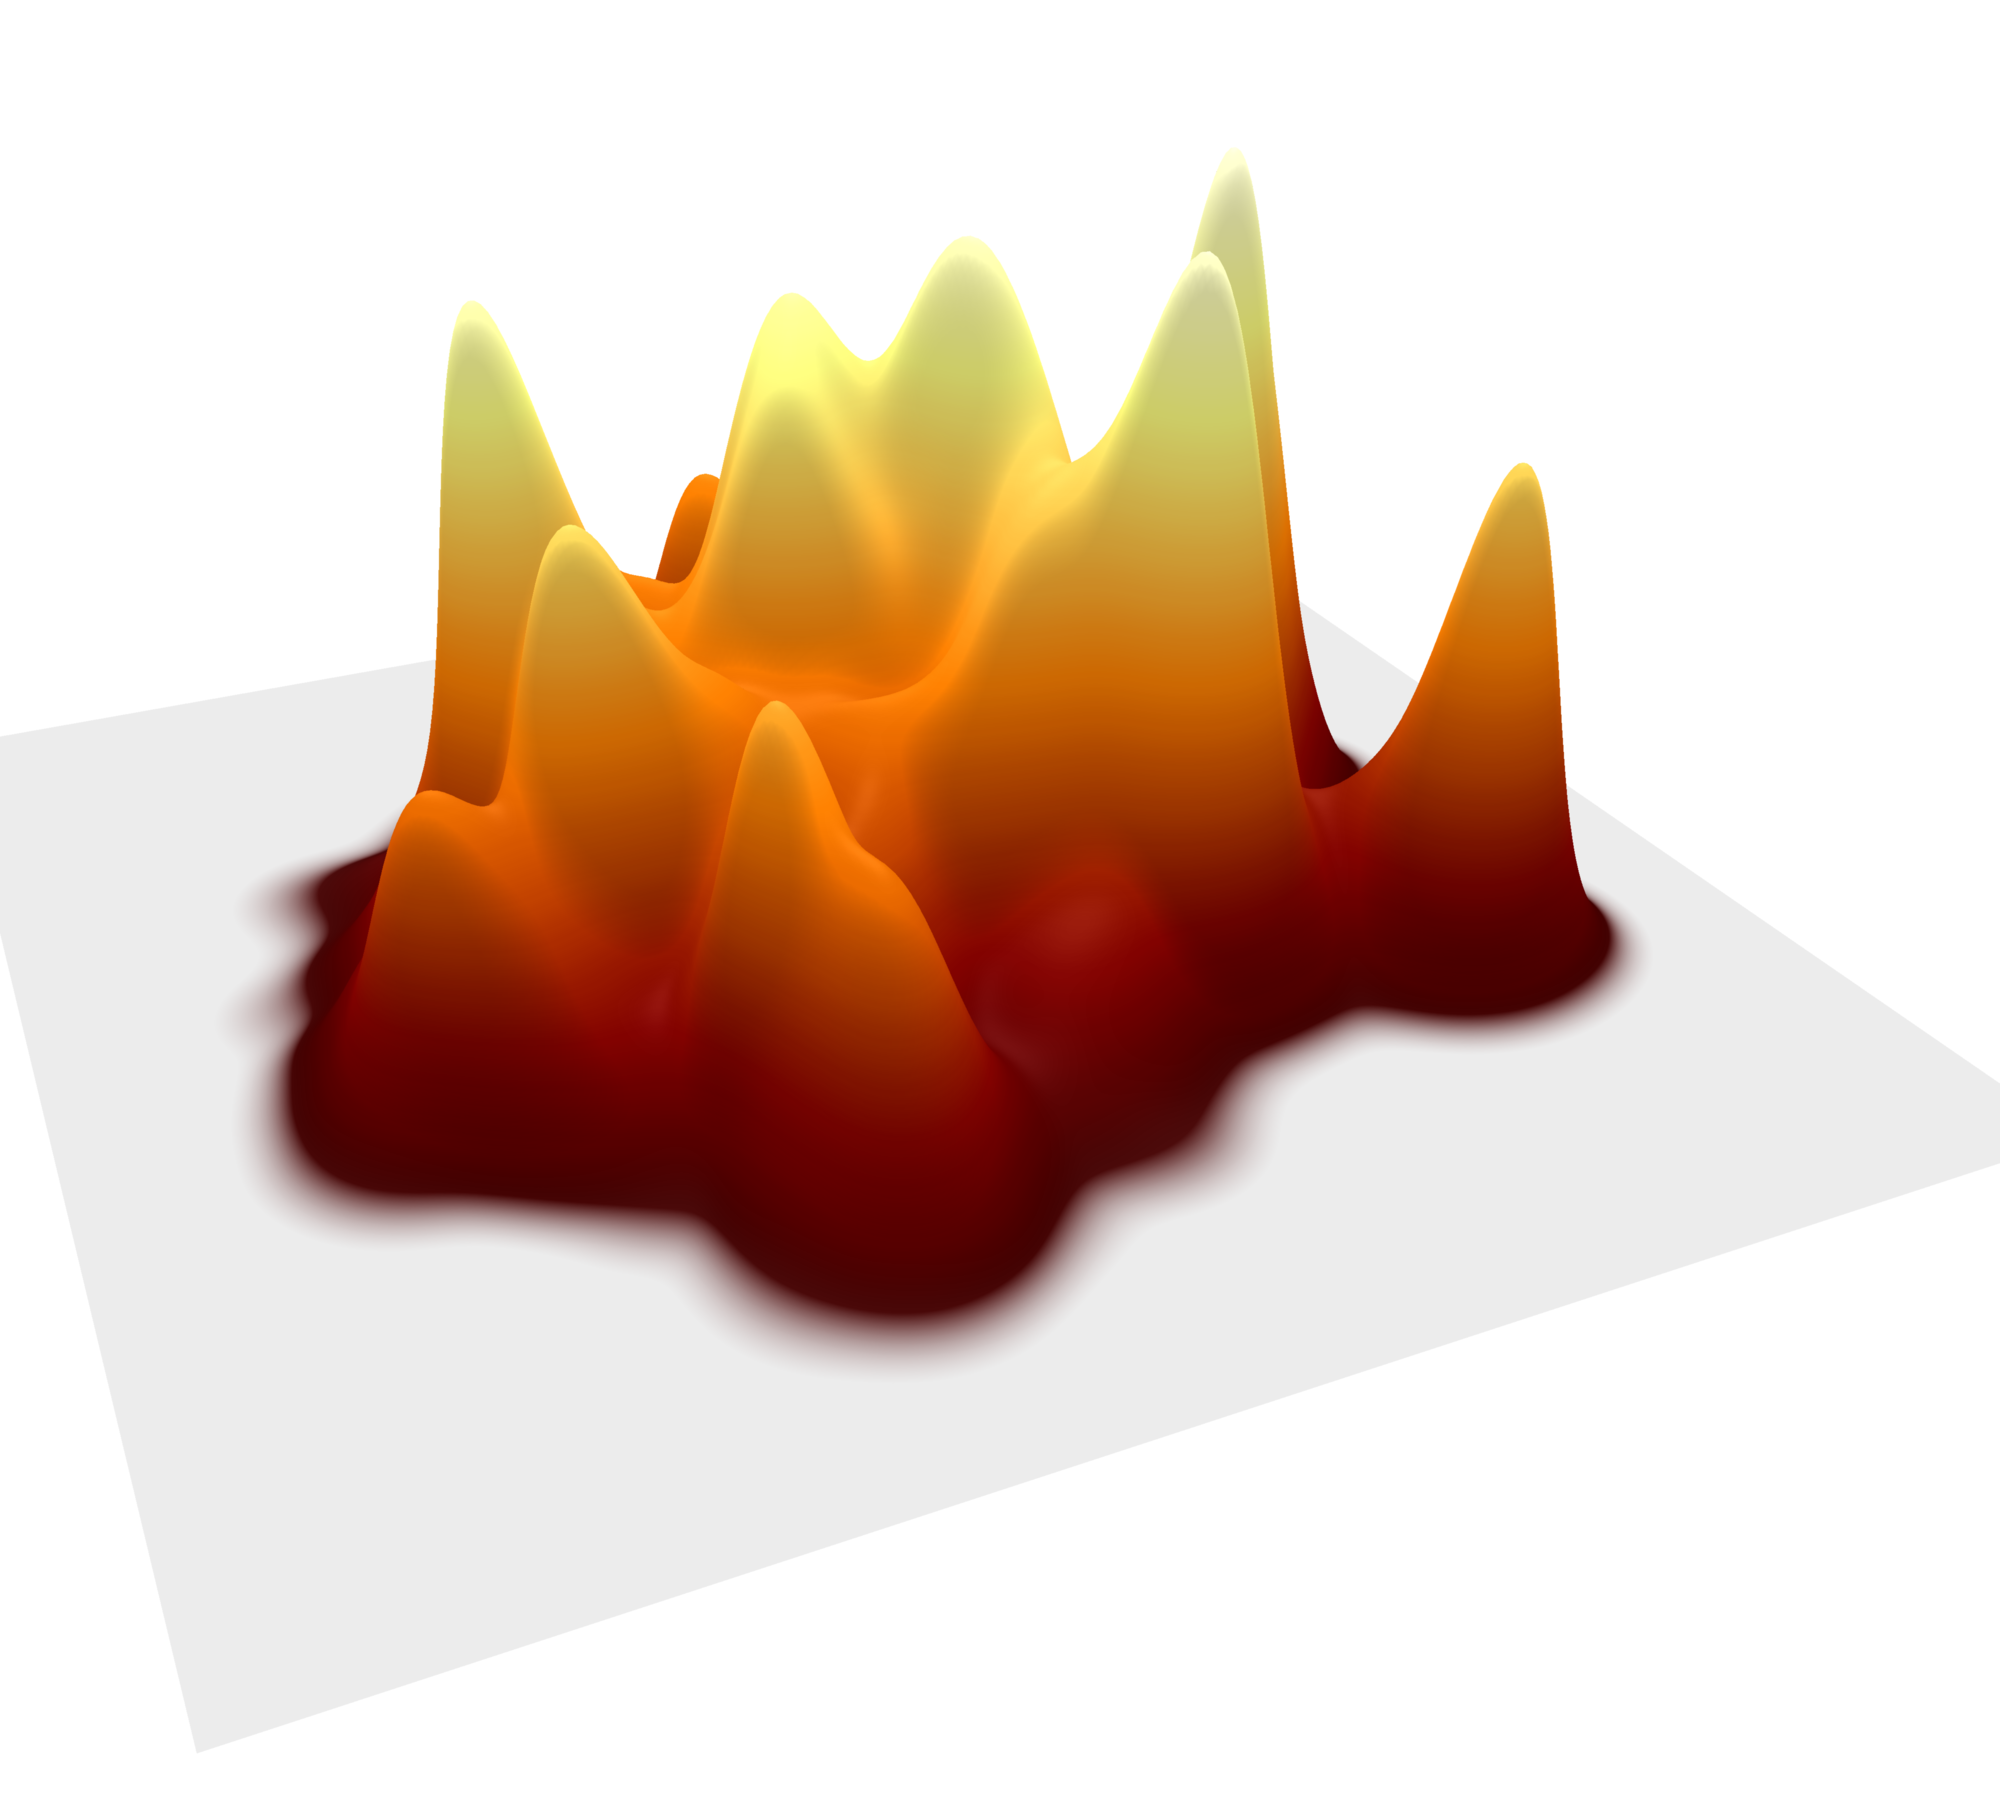
\includegraphics[width=\paperwidth]{trento2}};
}

\frame[plain,noframenumbering]{
  \begin{tikzpicture}[remember picture,overlay]
    \coordinate (middle) at (current page.center);
    \def\sep{.028\paperwidth}
    \def\extra{.6em}
    \node[rectangle, fill=theme, align=center, anchor=center, yshift=2.75cm, fill opacity=0.05, text opacity=1] at (middle) {
      \color{theme}\Large
      Determining QGP initial conditions and medium\\
      \color{theme}\Large
      properties with Bayesian analysis
    };
    %\def\extra{.25ex}
    \node[align=center, anchor=center, yshift=1. cm] at (middle) {
      \insertauthor \\[\extra]
      Initial Stages~$\vert$~\insertdate
    };
    \node[align=center, anchor=center, yshift=-3 cm] at (middle) {
      
\includegraphics[height=1.2cm]{qcdlogo} \hspace{0.2 cm} \hspace{0.2 cm}
      
\includegraphics[height=1.cm]{ssgf} \vspace{0.2 cm} \\
      \tiny Funding provided by DOE Stewardship Science Graduate Fellowship
    };
  \end{tikzpicture}
}

\usebackgroundtemplate{}

\begin{frame}{Reverse engineering IC from experiment}
    \vfill
    \begin{center}
    
    Objective is to constrain
    $\frac{dS}{d^2r_\perp dy} \propto f(\underbrace{T_A, T_B}_{\text{\tiny thickness}})$ \\ 
    
    \vspace{0.5 cm}

    using centrality dependent observables:\\
    
    \vspace{0.2 cm}
    
    yields $dN_\text{ch}/dy$, \quad mean $p_T$,\quad flow $v_n\{m\}$, \\
    
    \vspace{0.8 cm}
    
    and available collision systems:\\
 
    \vspace{0.3 cm}

    \small
    \begin{tabular}{cccccc}
        \multicolumn{6}{c}{200 GeV} \\ 
        \hline
        U+U & Au+Au & Cu+Cu & Cu+Au & d+Au & p+p
    \end{tabular} \\
    \vspace{0.4 cm}
    \begin{tabular}{ccc}
        \multicolumn{3}{c}{2.76 \& 5.02 TeV} \\
        \hline
        Pb+Pb & p+Pb & p+p
    \end{tabular}

    \end{center}
\end{frame}

\begin{frame}{Simplifying initial conditions}
    Start by defining local entropy (or energy) deposition in the eikonal approximation, 
    \begin{equation*}
        \frac{dS}{d^2r_\perp dy} \biggr \vert_{\sqrt{s_{NN}}} = \text{Norm} \cdot f(T_\text{part, A}, T_\text{part, B})
    \end{equation*}\\
    \vspace{0.1 cm}
    
    Mapping should only respect matter \underline{in the cross section} and hence,
    \begin{equation*}
        T_\text{part}(\vec{x}) = \sum\limits_{i=1}^{N_\text{part}} T_p(\vec{x} - \vec{x}_i)
    \end{equation*}
    In general, the normalization and mapping $f(T_\text{part, A}, T_\text{part, B})$ could have some dependence on $\sqrt{s_{NN}}$.
\end{frame}

\begin{frame}{Proposals for the mapping f}
    Two-component "Glauber" ansatz: \\
    \begin{flalign*}
        f = (1 - \alpha)\underbrace{\frac{T_{\text{part}, A} +  T_{\text{part}, B}}{2}}_{\text{arithmetic mean}} 
          + \alpha\, \underbrace{\sigma_{NN} T_{\text{part}, A}\, T_{\text{part}, B}}_{\text{quadratic term}}, 
    \end{flalign*}

    Original KLN model: \\
    \begin{align*}
        f &\sim Q^2_{s, \text{min}}\biggr[2 + \log\biggr(\frac{Q^2_{s,\text{max}}}{Q^2_{s, \text{min}}}\biggr)\biggr] \\
          &\sim T_\text{part,min} \biggr[2 + \log\biggr(\frac{T_\text{part,max}}{T_\text{part,min}}\biggr)\biggr] \\
    \end{align*}
\end{frame}

\begin{frame}{\trento\ initial condition model}
    Cat!
\end{frame}


\begin{frame}{Calibrating the model}
    \vfill
    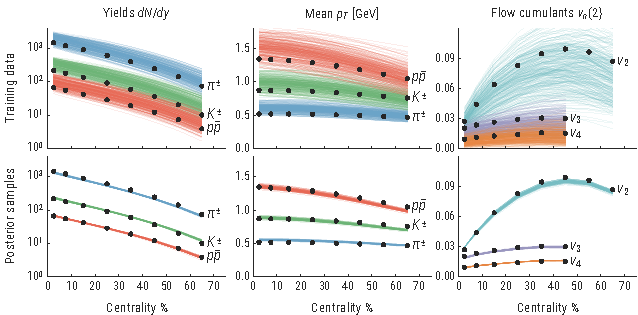
\includegraphics[width=\textwidth]{observables_plot}
\end{frame}

\begin{frame}{Running the model with high-likelihood parameters}
    \vfill
    \centering
    \scriptsize
    \begin{columns}
        \begin{column}{0.4\textwidth}
            Choose high likelihood \\model parameters
        \end{column}
        \begin{column}{0.6\textwidth}
            \begin{tabular}{lllll}
                \multicolumn{2}{c}{Initial condition} & & \multicolumn{2}{c}{QGP medium} \\
                \noalign{\smallskip}\hline\noalign{\smallskip}
                norm & 120.          &&  $\eta/s$ min   & 0.08       \\
                $p$  & 0.0           &&  $\eta/s$ slope & 0.85 GeV$^{-1}$   \\
                $k$  & 1.5           &&  $\zeta/s$ norm & 1.25       \\
                $w$  & 0.43 fm       &&  $T_\text{sw}$  & 0.148 GeV  \\
            \end{tabular}
        \end{column}
    \end{columns}
    \vspace{0.5 cm}
    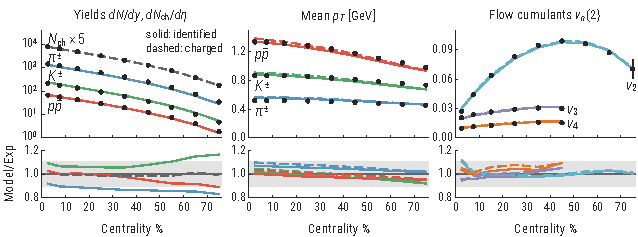
\includegraphics[width=\textwidth]{mode_observables} \\
    \vspace{0.2 cm}
    No emulator! Results represent actual hydro + UrQMD calculations!
\end{frame}

\begin{frame}
    \begin{columns}
        \begin{column}{0.2\textwidth}
            \vspace{-0.8 cm}
            \flushright \scriptsize
            \textcolor{gray}{dS/dy prefactor} \\
            \vspace{0.67 cm}
            \textcolor{gray}{Saturation intens.} \\
            \vspace{0.67 cm}
            \textcolor{gray}{p+p fluctuation} \\
            \vspace{0.67 cm}
            \textcolor{gray}{Nucleon width} \\
            \vspace{0.67 cm}
            \textcolor{gray}{$\eta/s$ minimum} \\
            \vspace{0.67 cm}
            \textcolor{gray}{$\eta/s$ slope} \\
            \vspace{0.67 cm}
            \textcolor{gray}{$\zeta/s$ norm} \\
            \vspace{0.67 cm}
            \textcolor{gray}{Switching temp}
        \end{column}
        \begin{column}{0.8\textwidth}
            \includegraphics[width=\columnwidth]{posterior_identified}
        \end{column}
    \end{columns}
\end{frame}

\begin{frame}
    \includegraphics[width=\textwidth]{nch_per_npart_2}
\end{frame}

\begin{frame}{Conclusions}
Yields, mean $p_T$ and flows impose strong constraints on IC. \\
Entropy  deposition mimic'd by $dS/dy \sim \sqrt{T_A T_B}$ \\
Data strongly prefers small nucleon width $w \approx 0.43$ fm! \\
A+A collisions weakly sensitivie to p+p mult.\ fluctuations \\
Prefered initial conditions similar to EKRT, IP-Glasma \\


\end{frame}
\end{document}
